    
\subsection*{Analytical Calculations}



\subsubsection*{Initialize}

\begin{verbatim}
close all; clear all; clc;

% Variables and Constants

mu_0 = 4*pi*1e-7;
depth = 20e-3; %m
g1 = 0.5e-3; %m
r0 = 12.5e-3; %m
r1 = 12e-3; %m
g2 = 2.5e-3; %m
r2 = 10e-3; %m
L = 20e-3; %m
N = 250; %turns
I = 3; %Amps
\end{verbatim}
\begin{par}
Reluctance of the system varies over a period. Maximum reluctance position is where the airgap is 2x2.5 mm, i.e. the rotor is in horizontal position. To find the varying reluctance over a period, following angles are defined (see angles.png):
\end{par} \vspace{1em}
\begin{verbatim}
a = asin(7.5/12); %rad
b = asin(7.5/12.5); %rad

alpha = pi/2-(a+b); %rad
\end{verbatim}


\subsubsection*{Reluctance and Inductance Definitions}

\begin{par}
Alpha is the angle where reluctance starts increasing, with respect to flux area, as a function of rotation angle. When rotor angle is alpha, corner of the salient part of the rotor is aligned with the corner of the stator. The change in the reluctance of the straight part of the rotor is ignored.
\end{par} \vspace{1em}
\begin{par}
Reluctance of the system can be defined as a pwl function.
\end{par} \vspace{1em}
\begin{par}
Reluctance for $\theta = 0:\alpha$ and $\theta = 180-\alpha:180$
\end{par} \vspace{1em}
\begin{verbatim}
Rel_min = @(thet) (2*g2)/(mu_0*(2*b-thet)*r0*L);
\end{verbatim}
\begin{par}
Reluctance for $\theta = \alpha:90$
\end{par} \vspace{1em}
\begin{verbatim}
Rel_rise = @(thet) (2*g1)/(mu_0*r1*(thet-alpha)*L);
\end{verbatim}
\begin{par}
Reluctance for $\theta = 90:180-\alpha$
\end{par} \vspace{1em}
\begin{verbatim}
Rel_fall = @(thet) (2*g1)/(mu_0*r1*(pi-alpha-thet)*L);

L_min = @(thet) N^2./Rel_min(thet);

L_rise = @(thet) N^2./(1/Rel_rise(thet)+1/Rel_min(thet-alpha))^(-1);

L_fall = @(thet) N^2./(1/Rel_fall(thet)+1/Rel_min(pi-alpha-thet))^(-1);
\end{verbatim}


\subsubsection*{Plot the Reluctance}

\begin{verbatim}
rot_angle = linspace(0,pi,1000);
Reluctance = zeros(1,length(rot_angle));

for i=1:length(rot_angle)
    t = rot_angle(i);
    if(t<=alpha)
        Reluctance(i) = Rel_min(0);
    end
    if(t>alpha && t<=pi/2)
        Reluctance(i) = Rel_rise(t);
    end
    if (t>pi/2 && t<=(pi-alpha))
        Reluctance(i) = Rel_fall(t);
    end
    if (t>(pi-alpha) && t<=(pi))
        Reluctance(i) = Rel_min(0);
    end

end

rot = linspace(0,2*pi,2000);
Rel_full_rot = [Reluctance,Reluctance];


figure;
plot(rot,Rel_full_rot,'LineWidth',2);
grid minor;
xlabel('Rotation Angle (rad)','FontSize',16);
ylabel('Reluctance (1/H)','FontSize',16);
ylim([0 5e7]);
title('Reluctance of the System','FontSize',16);
saveas(gcf,'Reluctance_analytical','epsc');
\end{verbatim}
\begin{center}
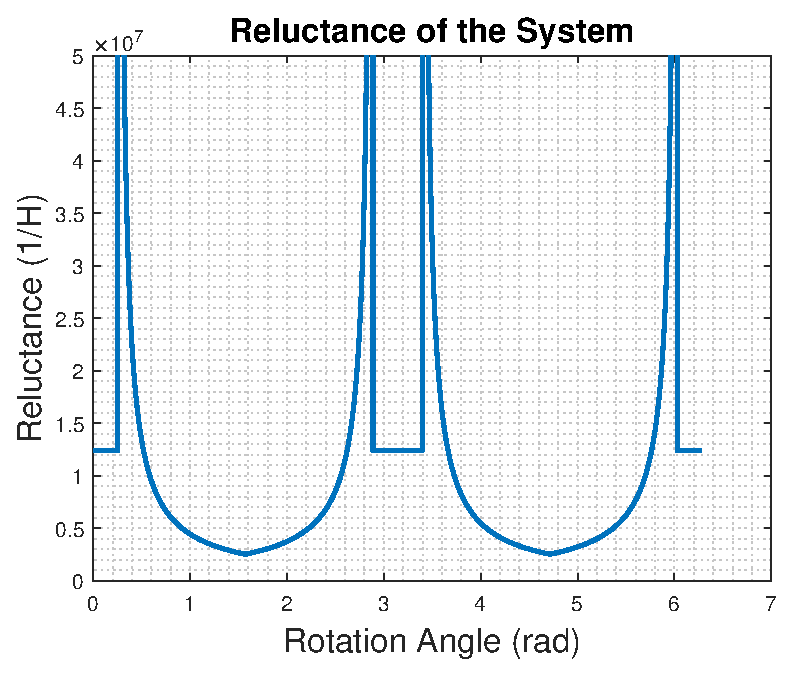
\includegraphics[width=4in]{html/analytical_01.eps}
\end{center}



\subsubsection*{Plot the Inductance}

\begin{verbatim}
rot_angle = linspace(0,pi,1000);
Inductance = zeros(1,length(rot_angle));

for i=1:length(rot_angle)
    t = rot_angle(i);
    if(t<=alpha)
        Inductance(i) = L_min(0);
    end
    if(t>alpha && t<=pi/2)
        Inductance(i) = L_rise(t);
    end
    if (t>pi/2 && t<=(pi-alpha))
        Inductance(i) = L_fall(t);
    end
    if (t>(pi-alpha) && t<=(pi))
        Inductance(i) = L_min(0);
    end

end

rot = linspace(0,2*pi,2000);
Ind_full_rot = [Inductance,Inductance];


figure;
plot(rot,Ind_full_rot,'LineWidth',2);
grid minor;
xlabel('Rotation Angle (rad)','FontSize',16);
ylabel('Inductance (H)','FontSize',16);
ylim([0 0.03]);
title('Inductance of the System','FontSize',16);
saveas(gcf,'inductance_analytical','epsc');
\end{verbatim}

\begin{center}

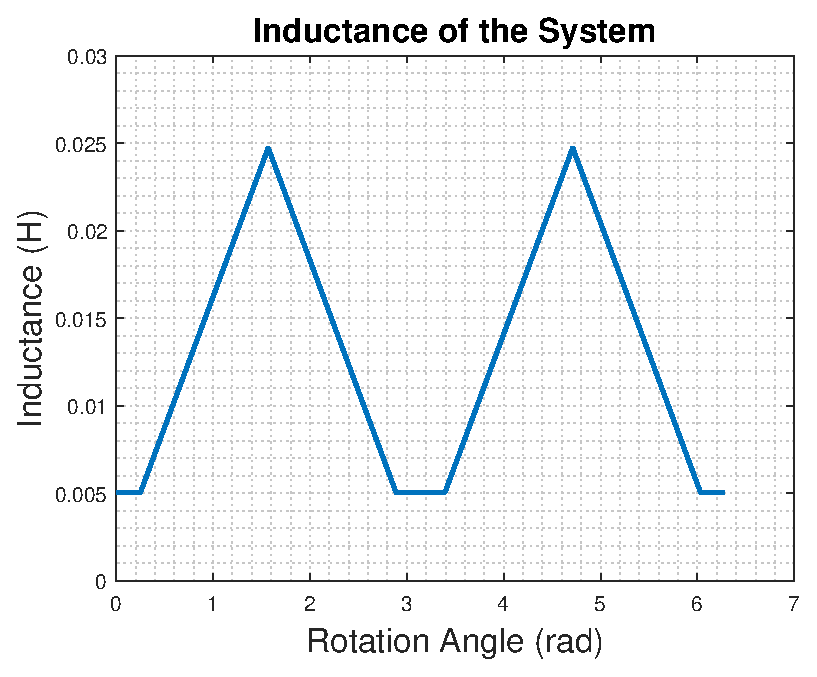
\includegraphics [width=4in]{html/analytical_02.eps}

\end{center}

\subsubsection*{Torque Calculation}

\begin{par}
$T = \frac{1}{2}\cdot I^2\cdot\frac{dL(\theta)}{d\theta}$
\end{par} \vspace{1em}
\begin{verbatim}
Torque_full_rot = zeros(size(Ind_full_rot));

for i = 1:length(Torque_full_rot)-1
    Torque_full_rot(i+1) = (Ind_full_rot(i+1)-Ind_full_rot(i))/(rot(i+1)-rot(i));
end

Torque_full_rot = Torque_full_rot*I^2/2;

figure;
plot(rot,Torque_full_rot,'LineWidth',2);
grid minor;
xlabel('Rotation Angle (rad)','FontSize',16);
ylabel('Torque (Nm)','FontSize',16);
% ylim([0 0.03]);
title('Torque of the Rotor','FontSize',16);
saveas(gcf,'torque_analytical','epsc');
\end{verbatim}

\begin{center}

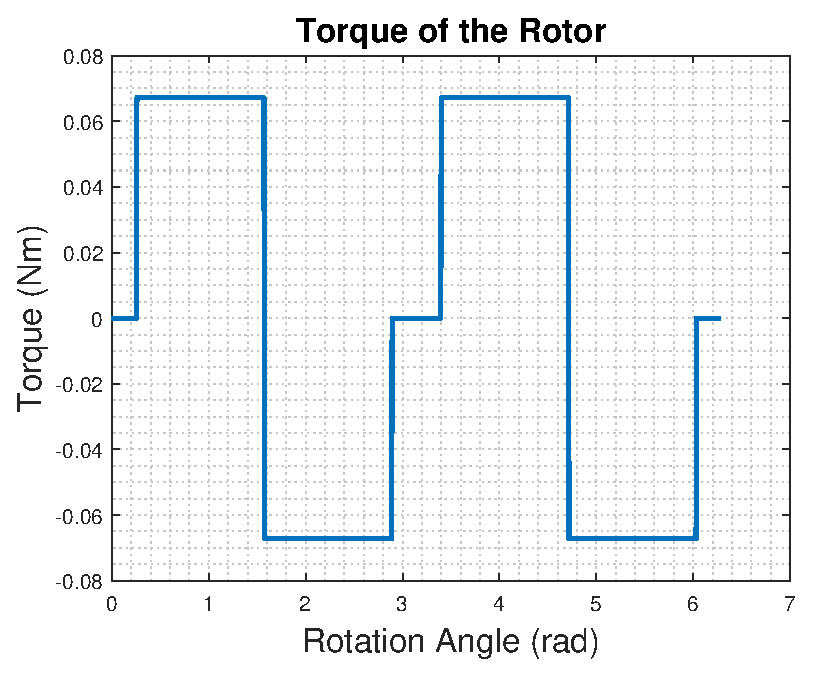
\includegraphics [width=4in]{html/analytical_03.eps}

\end{center}

